\documentclass[14pt]{extarticle}
\usepackage[utf8]{inputenc}
\usepackage[T1]{fontenc}
\usepackage[spanish,es-lcroman]{babel}
\usepackage{amsmath}
\usepackage{amsthm}
\usepackage{physics}
\usepackage{tikz}
\usepackage{float}
\usepackage{cancel}
\usepackage[autostyle,spanish=mexican]{csquotes}
\usepackage[per-mode=symbol]{siunitx}
\usepackage{gensymb}
\usepackage{multicol}
\usepackage{enumitem}
\usepackage{stackengine}
\usepackage{stix}
\usepackage[left=2.00cm, right=2.00cm, top=2.00cm, 
     bottom=2.00cm]{geometry}

\usepackage{Estilos/ColoresLatex}
\usepackage{makecell}
\usepackage{wrapfig}
\usepackage{titlesec}
\newcommand{\sectionbreak}{\clearpage}

\newcommand{\textocolor}[2]{\textbf{\textcolor{#1}{#2}}}
%\renewcommand{\questionlabel}{\thequestion)}

\newcommand{\Cancel}[2][black]{{\color{#1}\cancel{\color{black}#2}}}

\newcommand\deci[1]{%
    \kern-.4ex\stackunder[0.4pt]{$#1$}{$\color{blue}\acwunderarcarrow$}
}

\newcommand\decposl[1]{%    <--- Decimal position to left
    \kern-.4ex\stackunder[0.4pt]{$#1$}{%
      \reflectbox{$\color{red}\kern-.6ex\acwunderarcarrow$}
      }
}

\decimalpoint
\sisetup{bracket-numbers = false}

\title{\vspace*{-2cm} Guía de estudio 2do. examen parcial  Física III}
\author{M. en C. Ramón Gustavo Contreras Mayén \\ {\fontsize{14}{14}\selectfont Universidad del Valle de México. Campus San Rafael}}
% \institute{Universidad del Valle de México. Campus San Rafael.}
\date{}

\begin{document}
\maketitle


\section{Movimiento uniformemente acelerado.}

Cuando se resuelven problemas donde esté involucrada una \textocolor{red}{aceleración constante},  es importante elegir la fórmula correcta y sustituir los datos conocidos.

Los problemas se refieren frecuentemente al movimiento de un móvil que \textocolor{ao}{parte del reposo} (es decir, la $v_{i} = 0$, o que el móvil \textocolor{cadmiumgreen}{se detiene} (ahora la $v_{f} = 0$) después de cierta velocidad.

Las siguientes son las fórmulas más utilizadas en el movimiento uniformemente acelerado, entre corchetes se indican las unidades:
\begin{enumerate}
\item \textbf{Aceleración y tiempo. }Conociendo la velocidad final $v_{f}$, la velocidad inicial $v_{i}$ y el tiempo $t$, calculamos la aceleración del objeto:
\begin{align*}
a = \dfrac{v_{f} - v_{i}}{t} \hspace*{1.5cm} \left[ \dfrac{\unit{\meter}}{\unit{\square\second}} \right]
\end{align*}
\item \textbf{Aceleración y desplazamiento. } Conociendo la velocidad final $v_{f}$, la velocidad inicial $v_{i}$ y el desplazamiento $d$, calculamos la aceleración del objeto:
\begin{align*}
a = \dfrac{v_{f}^{2} - v_{i}^{2}}{2 \, d} \hspace*{1.5cm} \left[ \dfrac{\unit{\meter}}{\unit{\square\second}} \right]
\end{align*}
\item \textbf{Desplazamiento y tiempo. } Conociendo la velocidad final $v_{f}$, la velocidad inicial $v_{i}$ y el tiempo $t$, calculamos el desplazamiento que recorre el objeto:
\begin{align*}
d = \left( \dfrac{v_{f} + v_{i}}{2} \right) \, t \hspace*{1.5cm} \left[ \unit{\meter} \right]
\end{align*}
\item \textbf{Desplazamiento y aceleración. } Conociendo la la velocidad inicial $v_{i}$, la aceleración $a$ y el tiempo $t$, calculamos el desplazamiento que recorre el objeto:
\begin{align*}
d = v_{i} \, t + \dfrac{1}{2} \, a \, t^{2} \hspace*{1.5cm} \left[ \unit{\meter} \right]
\end{align*}
\end{enumerate}

\subsection{Ejercicios.}

\noindent
\textbf{Enunciado del ejercicio 1. } Una tren viaja a una velocidad de \SI{32}{\meter\per\second} y se detiene por completo después de haber recorrido \SI{140}{\meter}. 

¿Cuál fue su aceleración y en cuánto tiempo se detuvo?

\textocolor{red}{Solución al ejercicio. } El enunciado nos pide dos cosas:
\begin{enumerate}
\item La aceleración $a$.
\item El tiempo $t$ que tarda en detenerse.
\end{enumerate}

\textocolor{red}{Datos:}

\vspace*{0.5cm}
\begin{minipage}[t]{0.4\linewidth}
\begin{align*}
v_{i} &= \SI{32}{\meter\per\second} \\[0.2em]
v_{f} &= 0 \\[0.2em]
d &= \SI{140}{\meter}
\end{align*}
\end{minipage}
\hspace{1cm}
\begin{minipage}[t]{0.4\linewidth}
Incógnitas:
\begin{align*}
a &= \, ? \\[0.2em]
t &= \, ?
\end{align*}
\end{minipage}

\textocolor{red}{Expresiones a utilizar. } Este ejercicio requiere de dos expresiones.
 
\begin{eqnarray*}
\begin{aligned}
a &= \dfrac{v_{f}^{2} - v_{i}^{2}}{2 \, d} \\[0.5em] 
d &= \left( \dfrac{v_{f} + v_{i}}{2} \right) \, t  \hspace{0.2cm} \Rightarrow \hspace*{0.2cm} t = \dfrac{2 \, d}{v_{f} + v_{i}}
\end{aligned}
\end{eqnarray*}

\textocolor{red}{Sutitución:}
\begin{eqnarray*}
\begin{aligned}
a = \dfrac{ \left( \SI{0}{\meter\per\second} \right)^{2} - \left( \SI{32}{\meter\per\second} \right)^{2} }{2 ( \SI{140}{\meter})} = - \SI{3.66}{\meter\per\square\second}
\end{aligned}
\end{eqnarray*}

El signo negativo nos indica que hay una desaceleración o frenado, hemos resuelto la aceleración. Falta obtener el tiempo que transcurre para deternerse.
\begin{eqnarray*}
\begin{aligned}
t = \dfrac{2 (\SI{140}{\meter})}{\SI{32}{\meter\per\second} - \SI{0}{\meter\per\second}} = \SI{8.75}{\second}
\end{aligned}
\end{eqnarray*}

El tren tarda en detenerse completamente en \SI{8.75}{\second}, con esto hemos resuelto los dos incisos.

\vspace*{0.5cm}
\noindent
\textbf{Ejercicio 2.} Un caballo parte del reposo y alcanza una velocidad de \SI{15}{\meter\per\second} en un tiempo de \SI{8}{\second}. ¿Cuál fue su aceleración y qué distancia recorrió?

% \vspace*{0.5cm}
\begin{minipage}[t]{0.3\linewidth}
\textocolor{red}{Datos:}
\begin{align*}
v_{i} &= \SI{0}{\meter\per\second} \\
v_{f} &= \SI{15}{\meter\per\second} \\
t &= \SI{8}{\second} \\
\end{align*}
\end{minipage}
\hspace{0.1cm}
\begin{minipage}[t]{0.3\linewidth}
\hspace{1.5cm} Incógnitas:
\begin{align*}
a &= \, ? \\
d &= \, ?
\end{align*}
\end{minipage}

\vspace*{0.3cm}
\textocolor{red}{Expresiones:}
\begin{align*}
a = \dfrac{v_{f} - v_{i}}{t} \hspace{2cm}d = \left(\dfrac{v_{f} - v_{i}}{2} \right) \, t
\end{align*}

\vspace*{0.3cm}
\textocolor{red}{Sutitución:}

\vspace*{0.5cm}
Para la aceleración del caballo:
\begin{align*}
a = \dfrac{\displaystyle \SI[per-mode=fraction]{15}{\meter\per\second} - \SI[per-mode=fraction]{0}{\meter\per\second}}{\SI{8}{\second}} = \dfrac{\displaystyle \SI[per-mode=fraction]{15}{\meter\per\second}}{\SI{8}{\second}} = \SI[per-mode=fraction]{1.875}{\meter\per\square\second}
\end{align*}
Para el desplazamiento que realizó el caballo:
\begin{align*}
d = \left( \dfrac{\displaystyle \SI[per-mode=fraction]{0}{\meter\per\second} + \SI[per-mode=fraction]{15}{\meter\per\second}}{2} \right) \, (\SI{8}{\second})= \dfrac{ \SI{120}{\meter}}{2} = \SI{60}{\meter}
\end{align*}
El caballo tendrá una aceleración de \SI{1.875}{\meter\per\square\second} y recorrerá \SI{60}{\meter}.

\vspace*{0.5cm}
\noindent
\textbf{Enunciado del Ejercicio 3. } Una persona viaja en motocicleta a una velocidad de \SI{3}{\meter\per\second} y acelera constantemente a razón de \SI{0.4}{\meter\per\square\second} ¿Qué distancia recorrerá después de $1$ minuto? ¿Cuál será su velocidad final después de ese tiempo?

\begin{minipage}[t]{0.3\linewidth}
\textocolor{red}{Datos:}
\begin{align*}
v_{i} &= \SI{3}{\meter\per\second} \\
a &= \SI{0.4}{\meter\per\square\second} \\
t &= \SI{1}{\minute} = \SI{60}{\second}
\end{align*}
\end{minipage}
\hspace{0.1cm}
\begin{minipage}[t]{0.3\linewidth}
\hspace{1.5cm} Incógnitas:
\begin{align*}
d &= \, ? \\
v_{f} &= \, ?
\end{align*}
\end{minipage}

\vspace*{0.3cm}
\textocolor{red}{Expresiones:}
\begin{align*}
d &= v_{i} \, t + \dfrac{1}{2} \, a \, t^{2} \\[0.5em]
a &= \dfrac{v_{f} - v_{i}}{t} \hspace{2cm} \text{Despejamos la } v_{f} \\
a \, t &= v_{f} - v_{i} \\
v_{f} &= a \, t + v_{i}
\end{align*}

\vspace*{0.3cm}
\textocolor{red}{Sutitución:}

\vspace*{0.5cm}
Para la distancia recorrida:
\begin{align*}
d &= \left( \SI[per-mode=fraction]{3}{\meter\per\second} \right)(\SI{60}{\second}) + \dfrac{1}{2} \left(\SI[per-mode=fraction]{0.4}{\meter\per\square\second} \right)(\SI{60}{\second})^{2} = \\[0.5em]
d &= \SI{180}{\meter} + \dfrac{1}{2} \left(\SI[per-mode=fraction]{0.4}{\meter\per\square\second} \right)(\SI{3600}{\second}) = \\[0.5em]
d &= \SI{180}{\meter} + \dfrac{\SI{1440}{\meter}}{2} = \\[0.5em]
d &= \SI{180}{\meter} + \SI{720}{\meter} = \\[0.5em]
d &= \SI{900}{\meter}
\end{align*}

Para la velocidad final, tenemos que:
\begin{align*}
v_{f} &= \left( \SI[per-mode=fraction]{0.4}{\meter\per\square\second} \right) (\SI{60}{\second}) + \SI{3}{\meter} = \\[0.5em]
v_{f} &= \SI[per-mode=fraction]{24}{\meter\per\second} + \SI{3}{\meter} = \\[0.5em]
v_{f} &= \SI[per-mode=fraction]{27}{\meter\per\second}
\end{align*}
Esta persona recorrerá en la motocicleta una distancia de \SI{900}{\meter} con una velocidad final de \SI{27}{\meter\per\second}.

\section{Caída libre.}

Es bien sabido que, en ausencia de resistencia del aire, todos los objetos que se dejan caer cerca de la superficie de la Tierra caen hacia ella con la misma aceleración constante bajo la influencia de la gravedad de la Tierra.

Cuando se usa la expresión objeto en \textocolor{ao}{caída libre} no necesariamente se hace referencia a un objeto que se suelta desde el reposo.

Un objeto en caída libre es cualquier objeto que se mueve libremente sólo bajo la \textocolor{red}{influencia de la gravedad}, sin importar su movimiento inicial.

Los objetos que se lanzan hacia arriba o abajo y los que se liberan desde el reposo están todos en caída libre una vez que se liberan.

Cualquier objeto en caída libre experimenta una aceleración dirigida hacia abajo, sin importar su movimiento inicial.

La magnitud de la aceleración de caída libre se denota mediante el símbolo $g$. El valor de $g$ cerca de la superficie de la Tierra disminuye conforme aumenta la altitud, en la superficie de la Tierra, el valor de $g$ es aproximadamente \SI{9.81}{\meter\per\square\second}.

\subsection{Consideración importante.}

Si se ignora la resistencia del aire  y se supone que la aceleración de caída libre no varía con la altitud en distancias verticales cortas.

El movimiento de un objeto en caída libre que se mueve verticalmente es \textocolor{ao}{equivalente al movimiento de una partícula bajo aceleración constante en una dimensión}.

La \textocolor{carmine}{única modificación} que se necesita hacer en estas ecuaciones para los objetos en caída libre es notar que el movimiento es en la dirección vertical (la dirección $y$)  y que la aceleración es hacia abajo y tiene una magnitud de \SI{9.81}{\meter\per\square\second}

Ocupamos las ecuaciones desarrolladas que vimos para el M.U.A.

\begin{minipage}[t]{0.4\linewidth}
\begin{align*}
v_{f} &= v_{i} + g \, t \\[0.5em]
y &= \dfrac{1}{2} \big( v_{i} + v_{f} \big) \, t
\end{align*}
\end{minipage}
\hspace{1cm}
\begin{minipage}[t]{0.4\linewidth}
\begin{align*}
y &= v_{i} \, t + \dfrac{1}{2} g \, t^{2} \\[0.5em]
2 \, g \, y &= v_{f}^{2} - v_{i}^{2} 
\end{align*}
\end{minipage}

\vspace*{0.5cm}
En consecuencia,  siempre se elegirá:
\begin{align*}
a = - g = - \SI{9.81}{\meter\per\square\second}
\end{align*}
donde el signo negativo significa que la aceleración de un objeto en caída libre es hacia abajo.


\subsection{Ejercicios.}

\noindent
\textbf{Enunciado del Ejercicio 1. } Se deja caer una moneda de un peso desde la Torre Latinoamericana, parte del reposo y cae libremente. Calcula su posición y su velocidad después de $1.0$, $2.0$ y \SI{3.0}{\second}.
\begin{figure}[H]
\centering
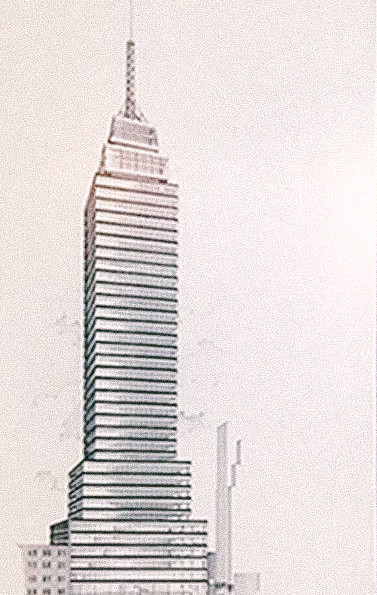
\includegraphics[scale=1.2]{Imagenes/Torre_Latino.jpg}
\end{figure}
\begin{tikzpicture}[overlay]
    \draw (7, 1.3) -- (7, 7) node [left, pos=1] {\small{$y$}};
    \draw (6, 1.3) -- (8, 1.3);
    \draw (6.7, 5.8) -- (7.3, 5.8);
    \draw [fill] (6.4, 5.8) circle (2pt);
\end{tikzpicture}

Para simplificar el estudio del problema, dejamos el esquema en donde se presenta el sistema de referencia del eje vertical y el objeto que cae.
\begin{figure}[H]
\centering
\begin{tikzpicture}
    \draw (7, -1) -- (7, 7) node [left, pos=1] {\small{$y$}};

    \node at (2, 4) {\small{$a = -g = - \SI{9.81}{\meter\per\square\second}$}};
    \draw [-stealth, thick] (2.5, 3.5) -- (2.5, 2.5);

    \draw (6, -1) -- (8, -1);
    \draw (6.7, 5.8) -- (7.3, 5.8);
    \draw [fill] (6.4, 5.8) circle (2pt);
    
    \node at (5.4, 5.6) {\small{$v_{i} = 0$}};
    \node at (8.5, 5.6) {\small{$t_{i} = 0 \quad y_{i}=0$}};
    
    \draw (6.7, 4.8) -- (7.3, 4.8);
    \draw [fill] (6.4, 4.8) circle (2pt);
    \node at (5.4, 4.6) {\small{$v_{1} =$ ?}};
    \draw [-stealth, thick] (6.4, 4.8) -- (6.4, 4.3);
    \node at (8.5, 4.6) {\small{$t_{1} = \SI{1}{\second} \quad y_{1}=$?}};
    
    \draw (6.7, 3) -- (7.3, 3);
    \draw [fill] (6.4, 3) circle (2pt);
    \draw [-stealth, thick] (6.4, 3) -- (6.4, 2.3);
    \node at (5.4, 2.8) {\small{$v_{2} =$ ?}};
    \node at (8.5, 2.8) {\small{$t_{2} = \SI{2}{\second} \quad y_{2}=$?}};

    \draw (6.7, 1) -- (7.3, 1);
    \draw [fill] (6.4, 1) circle (2pt);
    \draw [-stealth, thick] (6.4, 1) -- (6.4, -0.5);
    \node at (5.4, 0.8) {\small{$v_{3} =$ ?}};
    \node at (8.5, 0.8) {\small{$t_{3} = \SI{3}{\second} \quad y_{3}=$?}};

\end{tikzpicture}        
\end{figure}

Tomaremos el origen $O$ como el punto de partida y la dirección hacia arriba como positiva. La coordenada inicial $y_{0}$ y la velocidad inicial $v_{i}$ son ambas cero.

La aceleración es hacia abajo, en la dirección $y$ negativa,  así que:
\begin{align*}
a = - g = - \SI{9.81}{\meter\per\square\second}
\end{align*}
Recordemos que por definición, la magnitud de $g$ siempre es positiva.

Por lo que nuestras incógnitas son los valores de $y$ y $v$ en los tres instantes que indica el enunciado.

Tenemos las siguientes expresiones:
\begin{eqnarray*}
\begin{aligned}
y &= v_{i} \, t + \dfrac{1}{2} \, a \, t^{2} \\[0.5em] 
v &= v_{i} + a \, t 
\end{aligned}
\end{eqnarray*}

En un instante $t$ después de que se suelta la moneda, su posición y velocidad son:
\begin{eqnarray*}
\begin{aligned}
y &= 0 + \dfrac{1}{2} (-g) \, t^{2} = (\SI{-4.9}{\meter\per\square\second}) \, t^{2} \\[0.5em] 
v &= 0 + (-g) \, t = (\SI{-9.8}{\meter\per\square\second}) \, t
\end{aligned}
\end{eqnarray*}

Cuando $t = \SI{1}{\second}$, se tiene que:
\begin{eqnarray*}
\begin{aligned}
y &= (\SI{-4.9}{\meter\per\square\second}) \, (\SI{1}{\second})^{2} = \SI{-4.9}{\meter} \\[0.5em] 
v &= (\SI{-9.8}{\meter\per\square\second}) (\SI{1}{\second}) = \SI{-9.8}{\meter\per\second}
\end{aligned}
\end{eqnarray*}

Luego de \SI{1}{\second}, la moneda está \SI{4.9}{\meter} debajo del origen ($y$ es negativa),  y tiene una velocidad hacia abajo ($v$ es negativa) con magnitud de \SI{9.8}{\meter\per\second}.

La posición y velocidad a los \SI{2.0}{\second} y \SI{3.0}{\second} se obtienen de la misma manera. Se puede demostrar que:
\begin{table}[H]
\centering
\begin{tabular}{c | c | c}
Tiempo & Posición $(y)$ & Velocidad $(v)$ \\ \hline
\SI{2.0}{\second} & \SI{-19.6}{\meter} & \SI{-19.6}{\meter\per\second} \\ \hline
\SI{3.0}{\second} & \SI{-44.1}{\meter} & \SI{-29.4}{\meter\per\second} \\ \hline
\end{tabular}
\end{table}

\noindent
\textbf{Enunciado del Ejercicio 2. } Un niño lanza hacia abajo una piedra con una velocidad de \SI{2}{\meter\per\second} desde lo alto de un árbol de \SI{7}{\meter} de altura. 

Calcula en cuánto tiempo llegará al piso y con qué velocidad lo hará.

\begin{minipage}[t]{0.4\linewidth}
\textocolor{red}{Datos:}
\begin{align*}
v_{i} &= \SI{2}{\meter\per\second} \\[0.5em]
y &= \SI{7}{m} \\[0.5em]
g &= \SI{9.81}{\meter\per\square\second}
\end{align*}
\end{minipage}
\hspace{0.2cm}
\begin{minipage}[t]{0.4\linewidth}
Incógnitas
\begin{align*}
v_{f} = \, ? \\[0.5em]
t = \, ?
\end{align*}
\end{minipage}

\vspace*{0.5cm}
¿Qué expresión debemos de usar?

\vspace*{-1cm}
\begin{minipage}[t]{0.4\linewidth}
\begin{align*}
y &= \dfrac{1}{2} \big( v_{i} + v_{f} \big) \, t  \\[0.5em]
y &= v_{i} \, t + \dfrac{1}{2} g \, t^{2}
\end{align*}
\end{minipage}
\begin{minipage}[t]{0.4\linewidth}
\begin{align*}
v_{f} &= v_{i} + g \, t \\[0.5em]
2 \, g \, y &= v_{f}^{2} - v_{i}^{2} 
\end{align*}
\end{minipage}

Debemos de leer con cuidado el enunciado para identificar la expresión que nos será de utilidad.

\vspace*{0.5cm}
\noindent
\textocolor{red}{Expresiones:}

\noindent
Elegimos la siguiente expresión ya que involucra la $v_{f}$, pero notamos que no es una expresión \enquote{directa}, sino hay que despejar la velocidad final, que es la cantidad que nos piden:
\begin{eqnarray*}
\begin{aligned}
% y &= \dfrac{v_{f}^{2} - v_{i}^{2}}{2 \, g} [0.35em] 
2 \, g \, y &= v_{f}^{2} - v_{i}^{2} \\[0.35em] 
v_{f}^{2} &= 2 \, g \, y + v_{i}^{2} \\[0.35em] 
v_{f} &= \sqrt{2 \, g \, y + v_{i}^{2}} 
\end{aligned}
\end{eqnarray*}

La segunda expresión que nos devuelve el tiempo que tarda la piedra en llegar al piso, al conocer ya la velocidad con la que llega al suelo $v_{f}$, ocupamos la siguiente expresión de donde despejamos el tiempo $t$:

\vspace*{0.5cm}
\noindent
\textocolor{red}{Expresiones:}
\begin{align*}
v_{f} &= v_{i} + g \, t \\[0.5em] 
g \, t &= v_{f} - v_{i} \\[0.5em] 
t &= \dfrac{v_{f} - v_{i}}{g}
\end{align*}

Una vez conocidas las dos expresiones (recuerda que tenemos dos incógnitas), el siguiente paso es realizar la sustitución de los valores que nos da el enunciado.

\vspace*{0.5cm}
\noindent
\textocolor{red}{Sustitución:}

Para la velocidad:
\begin{align*}
v_{f} &= \sqrt{2 \left( \SI[per-mode=fraction]{9.81}{\meter\per\square\second} \right) \left( \SI{7}{\meter} \right) + \left( \SI[per-mode=fraction]{2}{\meter\per\second} \right)^{2}} = \\[0.4em] 
v_{f} &= \sqrt{\SI[per-mode=fraction]{137.34}{\square\meter\per\square\second} + \SI[per-mode=fraction]{4}{\square\meter\per\square\second}} = \sqrt{\SI[per-mode=fraction]{141.34}{\square\meter\per\square\second}} = \\[0.4em] 
v_{f} &= \SI[per-mode=fraction]{11.88}{\meter\per\second}
\end{align*}


\vspace*{0.5cm}
\noindent
Para obtener el tiempo:
\begin{align*}
t &= \dfrac{\displaystyle \SI[per-mode=fraction]{11.88}{\meter\per\second} - \SI[per-mode=fraction]{2}{\meter\per\second}}{\displaystyle \SI[per-mode=fraction]{9.81}{\meter\per\square\second}} = \\[0.6em] 
t &= \dfrac{\displaystyle \SI[per-mode=fraction]{9.88}{\meter\per\second}}{\displaystyle \SI[per-mode=fraction]{9.81}{\meter\per\square\second}} = \SI{1.007}{\second}
\end{align*}

Por lo que ahora conocemos que la piedra llega al suelo con una velocidad $v = \SI{11.88}{\meter\per\second}$ y tarda $t = \SI{1.007}{\second}$ en tocar el piso.

\vspace*{0.5cm}
\textbf{Enunciado del Ejercicio 3. } Calcula a) cuánto tiempo le tomó a King Kong caer desde la cima del edificio Empire State (\SI{380}{\meter} de altura) y b) cuál era su velocidad al \enquote{aterrizar}.

\begin{minipage}[t]{0.4\linewidth}
\textocolor{red}{Datos:}
\begin{align*}
v_{i} &= \SI{0}{\meter\per\second} \\[0.5em]
y &= \SI{380}{m} \\[0.5em]
g &= \SI{9.81}{\meter\per\square\second}
\end{align*}
\end{minipage}
\hspace{0.2cm}
\begin{minipage}[t]{0.4\linewidth}
Incógnitas
\begin{align*}
t = \, ? \\[0.5em]
v_{f} = \, ?
\end{align*}
\end{minipage}    

\vspace*{0.5cm}
\noindent
\textocolor{red}{Expresiones:}
\begin{eqnarray*}
\begin{aligned}
y &= v_{i} \, t + \dfrac{1}{2} \, g \, t^{2} \hspace{1cm} \text{Como } v_{i} = 0 \\[0.5em]
y &= \dfrac{1}{2} \, g \, t^{2} \hspace{1cm} \text{Despejamos el tiempo } t \\[0.5em]
2 \, y &= g \, t^{2} \\[0.5em]
t^{2} &= \dfrac{2 \, y}{g} \\[0.5em]
t &= \sqrt{\dfrac{2 \, y}{g}}
\end{aligned}
\end{eqnarray*}
De la expresión anterior ya se conocerá el tiempo qué tardó en caer King Kong, para conocer la velocidad con la que \enquote{aterriza}, ocupamos la siguiente expresión:

\noindent
\textocolor{red}{Expresiones:}
\begin{align*}
v_{f} &= v_{i} + g \, t \hspace{1cm} \text{Como } v_{i} = 0 \\[0.5em]
v_{f} &= g \, t
\end{align*}

\vspace{0.5cm}
\noindent
Para obtener el tiempo de caída: \\
\textocolor{red}{Sustitución:}
\begin{align*}
t &= \sqrt{\dfrac{2 \, (\SI{380}{\meter})}{ \displaystyle \SI[per-mode=fraction]{9.81}{\meter\per\square\second}}} = \\[0.5em]
t &= \sqrt{\dfrac{\SI{760}{\meter}}{\displaystyle \SI[per-mode=fraction]{9.81}{\meter\per\square\second}}} = \\[0.5em]
t &= \sqrt{ \SI{77.47}{\square\second}} = \\[0.5em]
t &= \SI{8.80}{\second}
\end{align*}

\vspace{0.5cm}
\noindent
Para obtener la velocidad con que llega al piso: \\
\textocolor{red}{Sustitución:}
\begin{align*}
v_{f} = \left( \SI[per-mode=fraction]{9.81}{\meter\per\square\second} \right) (\SI{8.80}{\second}) = \SI[per-mode=fraction]{86.32}{\meter\per\second}
\end{align*}

\section{Tiro vertical.}

Este movimiento se presenta cuando un objeto \textocolor{ao}{se lanza verticalmente hacia arriba}, y se observa que la magnitud de su \textocolor{armygreen}{velocidad va disminuyendo} hasta anularse al \textocolor{cadetblue!70!black}{alcanzar su altura máxima}.
\begin{figure}[H]
    \centering
    \begin{tikzpicture}
        \draw [-stealth] (0, 0) -- (0, 5) node [left, pos=1] {\small{$y$}};
        \draw (-1, 0) -- (4, 0);
        \node at (1.8, 0.2) {\small{$v_{0} > 0$}};
        \draw [-stealth] (1, 0.1) -- (1, 0.6);
        \draw [fill, color=ao] (1, 0.1) circle (0.1cm); 
        \draw [dashed] (1, 0.1) -- (1, 1.1);
        \draw [fill, color=ao] (1, 1.1) circle (0.1cm); 
        \draw [dashed] (1, 1.1) -- (1, 2.1);
        \draw [fill, color=ao] (1, 2.1) circle (0.1cm); 
        \draw [dashed] (1, 2.1) -- (1, 3.1);
        \draw [fill, color=ao] (1, 3.1) circle (0.1cm); 
        \draw [dashed] (1, 3.1) -- (1, 4.1);
        \draw [fill, color=ao] (1, 4.1) circle (0.1cm);
        \draw (-0.1, 4.1) -- (0.1, 4.1);
        \node at (-0.8, 4.1) {\small{$h = y_{\text{máx}}$}};
        \node at (1.8, 4.1) {\small{$v_{i} = 0$}};
    \end{tikzpicture}
\end{figure}
El tiempo que tarda en llegar al punto de máxima altura, se conoce como \textocolor{blue(pigment)}{tiempo de subida.}

Una vez que ha llegado al punto de máximo desplazamiento, inmediatamente inicia su regreso para llegar al mismo punto donde fue lanzado y adquiere la misma magnitud de velocidad con la cual partió.
\begin{figure}[H]
    \centering
    \begin{tikzpicture}
        \draw (0, 0) -- (0, 5)  node [left, pos=1] {\small{$y$}};;
        \draw (-1, 0) -- (4, 0);
        \draw [fill, color=ao] (1, 4.1) circle (0.1cm);
        \draw (-0.1, 4.1) -- (0.1, 4.1);
        \node at (-0.9, 4.1) {\small{$h = y_{\text{máx}}$}};
        \node at (1.8, 4.1) {\small{$v_{i} = 0$}};
        \draw [-stealth] (1, 4.1) -- (1, 3.6);
    \end{tikzpicture}
\end{figure}

Asimismo, el tiempo empleado en subir es el mismo utilizado en bajar, el tiempo total que el objeto está en movimiento, se conoce como \textocolor{bulgarianrose}{tiempo de vuelo}.

\subsection{Expresiones para el tiro vertical.}

El tiro vertical experimenta la misma aceleración que la caída libre de los objetos y, por tanto, emplea las mismas ecuaciones.

\begin{minipage}{0.4\linewidth}
\begin{align*}
v_{f} &= v_{i} + g \, t \\[0.5em]
y &= \dfrac{1}{2} \big( v_{i} + v_{f} \big) \, t
\end{align*}
\end{minipage}
\hspace{1cm}
\begin{minipage}{0.4\linewidth}
\begin{align*}
y &= v_{i} \, t + \dfrac{1}{2} g \, t^{2} \\[0.5em]
2 \, g \, y &= v_{f}^{2} - v_{i}^{2} 
\end{align*}
\end{minipage}   

\vspace*{0.5cm}
Para calcular la altura máxima que alcanza un objeto lanzado verticalmente hacia arriba usamos la ecuación:
\begin{align*}
h_{\text{máx}} = y_{\text{máx}} - \dfrac{v_{i}^{2}}{2 \, g}
\end{align*}
Revisa que en física, el valor de la altura máxima se puede escribir con $y$ o con $h$, pero representa la misma variable.

Para calcular el tiempo que tarda en subir (tiempo de subida) utilizamos la ecuación:
\begin{align*}
t_{\text{subida}} = - \dfrac{v_{i}}{g}
\end{align*}

Como el tiempo que tarda en subir es el mismo para bajar, entonces el tiempo de permanencia en el aire (tiempo de vuelo) será:
\begin{align*}
t_{\text{aire}} = - \dfrac{2 \, v_{i}}{g}
\end{align*}    

\subsection{Ejercicios de tiro vertical.}

\textbf{Ejercicio tiro vertical 1. } Un balón de voleibol que se encuentra al nivel del suelo es lanzado verticalmente hacia arriba con una velocidad de \SI{29.4}{\meter\per\second}.

\vspace*{0.5cm}
Calcula:
\begin{enumerate}
\item ¿Qué altura habrá subido al primer segundo?
\item ¿Qué magnitud de velocidad llevará al primer segundo?
\item ¿Qué altura máxima alcanzará?
\item ¿Qué tiempo tardará en subir?
\item ¿Cuánto tiempo durará en el aire?
\end{enumerate}
Toma en cuenta de que en un mismo enunciado se pueden pedir varias cantidades; se recomienda que se resuelvan en el mismo orden en el que se presentan.

Presentamos los datos que reconocemos del enunciado.

\vspace*{0.5cm}
\begin{minipage}[t]{0.4\linewidth}
\textocolor{red}{Datos:}
\begin{eqnarray*}
\begin{aligned}
v_{i} &= \SI{29.4}{\meter\per\second} \\
g &= \SI{9.81}{\meter\per\square\second}
\end{aligned}
\end{eqnarray*}
\end{minipage}
\hspace{1cm}
\begin{minipage}[t]{0.4\linewidth}
Incógnitas:
\begin{align*}
h_{1 \, s} &= \, ? \\
v_{1 \, s} &= \, ? \\
y_{\text{máx}} &= \, ? \\
t_{\text{subida}} &= \, ? \\ 
t_{\text{vuelo}} &= \, ?
\end{align*}
\end{minipage}

\vspace*{0.5cm}

\noindent
¿Qué altura habrá subido al primer segundo?

\textocolor{red}{Expresión:}
\begin{align*}
y = v_{i} \, t + \dfrac{g \, t^{2}}{2}
\end{align*}

Hacemos la sustitución para resolver esta pregunta.

\vspace*{0.5cm}
\textocolor{red}{Sustitución:}
\begin{align*}
y_{1 s} &= \left[ \left( \SI[per-mode=fraction]{29.4}{\meter\per\second} \right) (\SI{1}{\second}) \right] + \dfrac{\displaystyle \left( - \SI[per-mode=fraction]{9.8}{\meter\per\square\second} \right)(\SI{1}{\second})^{2}}{2} = \\[0.5em] 
y_{1 s} &= \SI{29.4}{\meter} - \SI[per-mode=fraction]{4.9}{\meter} = \\[0.5em] 
y_{1 s} &= \SI{24.5}{\meter}
\end{align*}

La altura que alcanza el balón en el primer segundo de movimiento es $y_{1 s} = \SI{24.5}{\meter}$

\vspace*{0.5cm}
¿Qué magnitud de velocidad llevará al primer segundo?. Como ya conocemos la velocidad al primer segundo, podemos llamar $v_{f}$ a esa cantidad, para así, usar la siguiente expresión:

\vspace*{0.5cm}
\textocolor{red}{Expresión:}
\begin{align*}
v_{f} = v_{i} + g \, t
\end{align*}

Pasamos al siguiente paso de la solución para este inciso:

\vspace*{0.5cm}
\textocolor{red}{Sustitución:}
\begin{align*}
v_{1 s} &= \left( \SI[per-mode=fraction]{29.4}{\meter\per\second}\right) + \left[ \displaystyle \left( - \SI[per-mode=fraction]{9.8}{\meter\per\square\second} \right) (\SI{1}{\second}) \right] = \\[0.5em]
v_{1 s} &= \SI[per-mode=fraction]{29.4}{\meter\per\second} - \SI[per-mode=fraction]{9.8}{\meter\per\second} = \\[0.5em]
v_{1 s} &= \SI[per-mode=fraction]{19.6}{\meter\per\second}
\end{align*}
La velocidad del objeto al primer segundo es $v_{1 \, s} = \SI{19.6}{\meter\per\second}$.

\vspace*{0.5cm}
\noindent
\textbf{Enunciado del ejercicio 2.}  Se batea una pelota casi en línea recta hacia arriba en el aire con una velocidad aproximada de \SI{20}{\meter\per\second}. Responde: a) ¿Qué tan alto sube? y b) ¿Cuánto tiempo permanece en el aire?

\vspace*{0.5cm}
\begin{minipage}[t]{0.3\linewidth}
\textocolor{red}{Datos:}
\begin{eqnarray*}
\begin{aligned}
v_{i} &= \SI{20.4}{\meter\per\second} \\
g &= \SI{9.81}{\meter\per\square\second}
\end{aligned}
\end{eqnarray*}
\end{minipage}
\hspace{1cm}
\begin{minipage}[t]{0.4\linewidth}
Incógnitas:
\begin{align*}
y_{\text{máx}} &= \, ? \\
t_{\text{vuelo}} &= \, ?
\end{align*}
\end{minipage}

\vspace*{0.5cm}
\textocolor{red}{Expresiones:}
\begin{align*}
y_{\text{máx}} = - \dfrac{v_{i}^{2}}{2 \, g} \hspace{1.5cm} t_{vuelo} = - \dfrac{2 \, v_{i}}{g}
\end{align*}

\vspace*{0.5cm}
\textocolor{red}{Sustitución:}

Para la altura máxima que alcanza la pelota:
\begin{align*}
y_{\text{máx}} &= - \dfrac{ \displaystyle\left( \SI[per-mode=fraction]{20}{\meter\per\second}\right)^{2}}{ \displaystyle - \SI[per-mode=fraction]{9.81}{\meter\per\square\second}} = \dfrac{\displaystyle \SI[per-mode=fraction]{400}{\square\meter\per\second}}{\displaystyle \SI[per-mode=fraction]{9.81}{\meter\per\square\second}} = \\[0.5em]
y_{\text{máx}} &= \SI{40.77}{\meter}
\end{align*}

\vspace*{0.3cm}
Para el tiempo de vuelo:
\begin{align*}
t_{\text{vuelo}} = - \dfrac{2 \, \left( \displaystyle \SI[per-mode=fraction]{20}{\meter\per\second} \right)}{\displaystyle - \SI[per-mode=fraction]{9.81}{\meter\per\square\second}} = \SI[per-mode=fraction]{4.07}{\second}
\end{align*}


\section{Fuerza.}

En el lenguaje cotidiano, fuerza es un empujón o un tirón. Una \textocolor{byzantine}{fuerza} es una interacción entre dos cuerpos o entre un cuerpo y su ambiente.

La fuerza es una cantidad vectorial, por lo que tiene una magnitud, dirección y sentido.

\subsection{Tipos de fuerza.}

\begin{enumerate}
\item Una \textocolor{cobalt}{fuerza de contacto}, es aquella fuerza que implica un contacto directo entre dos cuerpos, como un empujón o un tirón.
\begin{figure}[H]
    \centering
    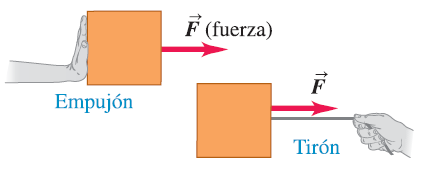
\includegraphics[scale=0.8]{Imagenes/Fuerza_01.png}
    \caption{Ejemplo de fuerza de contacto.}
\end{figure}
\item \textcolor{ao(english)}{Fuerzas de largo alcance.} Son aquellas fuerzas que actúan aunque los cuerpos estén separados.
\begin{figure}[H]
    \centering
    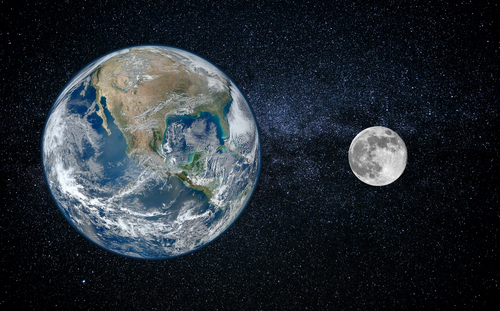
\includegraphics[scale=1.3]{Imagenes/Fuerza_09.jpg}
    \caption{Ejemplo de fuerzas a distancia.}
\end{figure}
\end{enumerate}

Recordemos que:
\begin{enumerate}
\item La masa de un objeto es la cantidad de sustancia que contiene un cuerpo, en el sistema MKS su unidad es el \unit{\kilo\gram}, en el sistema cgs, la unidad es el \unit{\gram}.
\item El peso  es la masa multiplicada por el valor de \textbf{g}, la aceleración debida a la gravedad: \SI{9.81}{\meter\per\square\second}, las unidades del peso son los Newtons (\unit{\newton})
\begin{align*}
\text{Peso} = m \, g \hspace{0.5cm} \Rightarrow \hspace{0.5cm} \left[ \unit{\newton} \right]
\end{align*}
\end{enumerate}

\subsection{Ejercicios de masa y peso.}

\textbf{Ejercicio 1.} Hallar la magnitud del peso de una roca cuya masa es de \SI{100}{\kilo\gram}.

Solución: Escribimos con la letra $W$ el peso, por lo que:
\begin{align*}
W = m \, g = (\SI{100}{\kilo\gram})(\SI{9.81}{\meter\per\square\second}) = \SI{981}{\newton}
\end{align*}
Las unidades de peso son los \textbf{Newtons} (\unit{\newton})

\vspace*{0.5cm}
\textbf{Ejercicio 2.}  Determina la masa de una roca cuyo peso tiene una magnitud de \SI{1500}{\newton}.

Solución:
\begin{align*}
m = \dfrac{W}{g} = \dfrac{\SI{1500}{\newton}}{\SI{9.81}{\meter\per\square\second}} = \SI{152.90}{\kilo\gram}
\end{align*}
Las unidades de masa son \textbf{kilogramos} (\unit{\kilo\gram})

\section{Las leyes de Newton}

\begin{wrapfigure}{R}{0.3\textwidth}
\centering
    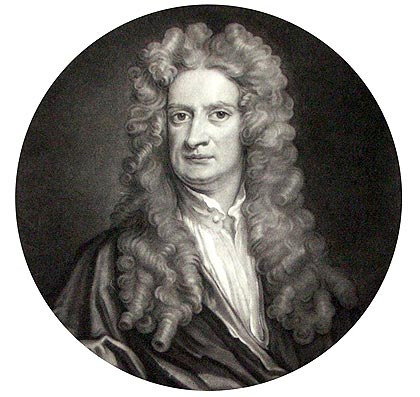
\includegraphics[scale=0.35]{Imagenes/Newton.jpg}
\end{wrapfigure}
El científico inglés Isaac Newton, estudió las leyes generales que rigen el movimiento de los objetos, observando la caída de una manzana al suelo, al establecer las relaciones entre la fuerza que provocó esta caída y la fuerza que sostiene a la Luna en su órbita alrededor de la Tierra.

Plasmó sus estudios en el libro \emph{Philosophiae Naturalis Principia Mathematica}, donde estableció las tres leyes del movimiento, también conocidas como leyes de Newton, base de lo que hoy conocemos como mecánica clásica o mecánica newtoniana, así como de ley de gravitación universal.

\subsection{Primera ley.}

\textocolor{carmine}{Ley de la inercia} Un cuerpo sobre el que no actúa una fuerza neta se mueve con velocidad constante (que puede ser cero) y aceleración cero.

Un objeto en reposo permanece en reposo o en movimiento, continuará en movimiento con una velocidad constante a menos que se aplique una fuerza externa neta para modificar dicho estado.

\begin{figure}[H]
    \centering
    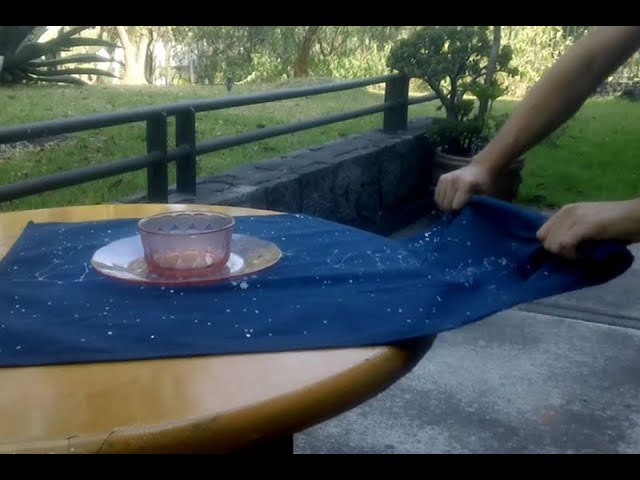
\includegraphics[scale=0.35]{Imagenes/Newton_01.jpg}
    \caption{Ejemplo de la primera ley de Newton.}
\end{figure}

La tendencia de un cuerpo a seguir moviéndose una vez iniciado su movimiento es resultado de una propiedad llamada \textocolor{darkmagenta}{inercia}.


\subsection{Segunda ley.}

Si una \textocolor{darkscarlet}{fuerza externa neta} actúa sobre un cuerpo, éste se acelera. La dirección de aceleración es la misma que la dirección de la fuerza neta. 

\textbf{Expresión para la segunda ley. } El vector de fuerza neta es igual a la masa del cuerpo multiplicada por su aceleración.
\begin{align*}
\va{F} = m \, \va{a}
\end{align*}

La segunda ley de Newton es una ley fundamental de la naturaleza, \textocolor{darkslateblue}{la relación básica entre fuerza y movimiento}.

Ocupamos una referencia gráfica para el uso de la segunda ley de Newton: \textocolor{debianred}{el triángulo de la fuerza}:
\begin{figure}[H]
    \centering
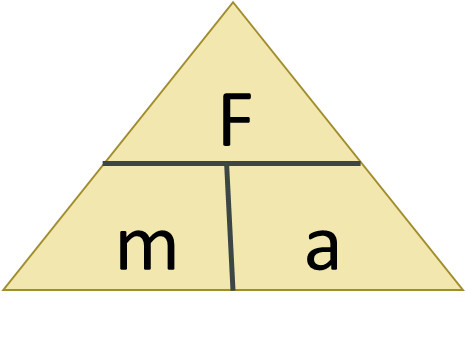
\includegraphics[scale=1.5]{Imagenes/Newton_11.jpg}
\end{figure}

% \textbf{Ejercicio con la segunda ley. } Un trabajador aplica una fuerza horizontal constante con magnitud de \SI{20}{\newton} a una caja con masa de \SI{40}{\kilo\gram} que descansa en un piso plano con fricción despreciable. ¿Qué aceleración experimenta la caja?.

% \begin{figure}[H]
%     \centering
%     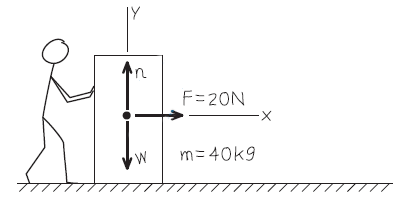
\includegraphics[scale=1]{Imagenes/Newton_02.png}
%     \caption{Esquema que nos plantea el ejercicio.}
% \end{figure}

% \vspace*{0.5cm}

% \begin{minipage}[t]{0.4\linewidth}
% \textocolor{red}{Datos:}
% \begin{align*}
% F &= \SI{20}{\newton} \\[0.5em]
% m &= \SI{40}{\kilo\gram}
% \end{align*}
% \end{minipage}
% \hspace{1cm}
% \begin{minipage}[t]{0.4\linewidth}
% \textocolor{red}{Expresión:}
% \begin{figure}[H]
%     \centering
%     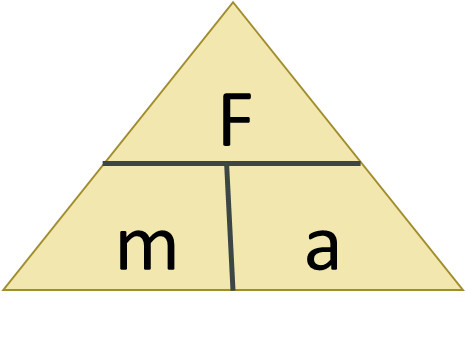
\includegraphics[scale=1]{Imagenes/Newton_11.jpg}
% \end{figure}

% \begin{align*}
% a = \dfrac{F}{m}
% \end{align*}
% \end{minipage}

% \vspace*{0.5cm}
% \textocolor{red}{Sustitución:}

% \begin{align*}
% a &= \dfrac{F}{m} = \dfrac{\SI{20}{\newton}}{\SI{40}{\kilo\gram}} = 0.5 \, \dfrac{\dfrac{\unit{\kilo\gram\meter}}{\unit{\square\second}}}{\unit{\kilo\gram}} = 0.5 \, \dfrac{\unit{\kilo\gram\meter}}{\unit{\kilo\gram\square\second}} = \SI[per-mode=fraction]{0.5}{\meter\per\square\second}
% \end{align*}

% Conviene aclarar que en el sistema \textbf{MKS}, se utilizan las unidades de metro, kilogramo y segundo, como unidades de longitud, masa y tiempo, respectivamente.

% En ciencia e ingeniería se utiliza también un sistema llamado \textbf{cgs}, donde las unidades de longitud, masa y tiempo son: el centímetro, gramo y segundo. La unidad de medida de la fuerza en el sistema \textbf{cgs}, es la llamada \textocolor{denim}{dina}:
% \begin{align*}
% 1 \, \text{dina} = \SI[per-mode=fraction]{1}{\gram\centi\meter\per\square\second}
% \end{align*}

% En el sistema británico, las unidades de:
% \begin{enumerate}
% \item Fuerza es la \textocolor{ao}{libra} (o libra-fuerza).
% \item Masa es el \textocolor{electricindigo}{slug}.
% \item Aceleración es el pie por segundo al cuadrado.
% \end{enumerate}

% Así que la unidad de fuerza en el sistema inglés es:
% \begin{align*}
% 1 \, \text{libra-fuerza} = \text{slug} \, \dfrac{\text{pie}}{\unit{\square\second}}
% \end{align*}

% \vspace*{0.5cm}
% \textbf{Enunciado del ejercicio 2. } Determina la fuerza que se necesita aplicar a un auto de \SI{800}{\kilo\gram} para que éste se acelere \SI{4}{\meter\per\square\second}.

% \vspace*{0.5cm}

% \begin{minipage}[t]{0.4\linewidth}
% \textocolor{red}{Datos:}
% \begin{align*}
% m &= \SI{800}{\kilo\gram} \\[0.5em]
% a &= \SI{4}{\meter\per\square\second} \\[0.5em]
% F &= \, ?
% \end{align*}
% \end{minipage}
% \hspace{1cm}
% \begin{minipage}[t]{0.4\linewidth}
% \textocolor{red}{Expresión:}
% \begin{figure}[H]
%     \centering
%     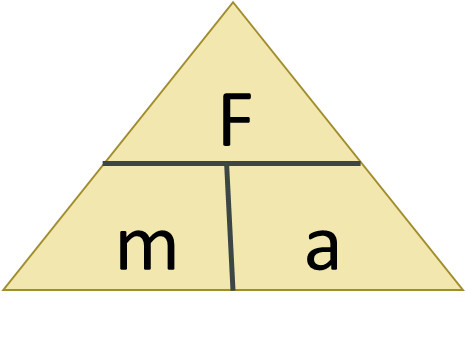
\includegraphics[scale=1]{Imagenes/Newton_11.jpg}
% \end{figure}

% \begin{align*}
% F = m \, a
% \end{align*}
% \end{minipage}

% \vspace*{0.5cm}
% \textocolor{red}{Sustitución:}

% \begin{align*}
% F &= \left( \SI{800}{\kilo\gram} \right) \left( \SI{4}{\meter\per\square\second} \right) = \\[0.5em]
% F &= \SI[per-mode=fraction]{3.2d3}{\kilo\gram\meter\per\square\second} = \SI{3.2d3}{\newton}
% \end{align*}

% \vspace*{0.5cm}

% \textbf{Enunciado del ejercicio 3. } El resultado de las fuerzas que actúan sobre un cuerpo cuya masa vale \SI{40}{\kilo\gram}, es de \SI{85}{\newton} ¿Cuál es el valor de la aceleración que posee este cuerpo?

% \vspace*{0.5cm}
% \begin{minipage}[t]{0.4\linewidth}
% \textocolor{red}{Datos:}
% \begin{align*}
% m &= \SI{40}{\kilo\gram} \\[0.5em]
% F &= \SI{85}{\newton} \\[0.5em]
% a &= \, ?
% \end{align*}
% \end{minipage}
% \hspace{1cm}
% \begin{minipage}[t]{0.4\linewidth}
% \textocolor{red}{Expresión:}
% \begin{figure}[H]
%     \centering
%     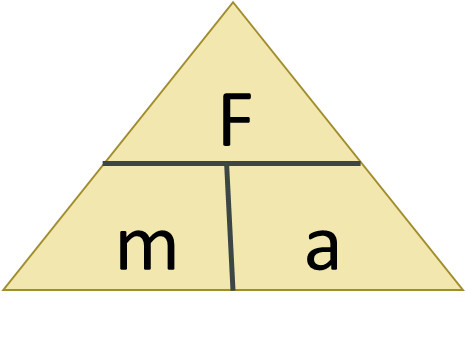
\includegraphics[scale=1]{Imagenes/Newton_11.jpg}
% \end{figure}
% \begin{align*}
% a = \dfrac{F}{m}
% \end{align*}
% \end{minipage}

% \vspace*{0.5cm}
% \textocolor{red}{Sustitución:}

% \begin{align*}
% a &= \dfrac{\SI{85}{\newton}}{\SI{40}{\kilo\gram}} = \\[0.5em]
% a &= 2.125 \, \dfrac{\dfrac{\unit{\kilo\gram\meter}}{\unit{\square\second}}}{\unit{\kilo\gram}} = 2.125 \, \dfrac{\unit{\kilo\gram\meter}}{\unit{\kilo\gram\square\second}} \\[0.5em]
% a &= \SI[per-mode=fraction]{2.125}{\meter\per\square\second}
% \end{align*}

% \textbf{Ejercicio más elaborado 4. } ¿Qué fuerza debe ejercer el motor de un automóvil cuya masa es de \SI{1500}{\kilo\gram} para aumentar su velocidad de \SI{4.5}{\kilo\meter\per\hour} a \SI{40}{\kilo\meter\per\hour} en \SI{8}{\second}?

% \vspace*{0.5cm}

% \begin{minipage}[t]{0.4\linewidth}
% \textocolor{red}{Datos:}
% \begin{align*}
% m &= \SI{1500}{\kilo\gram} \\[0.5em]
% F &= \, ? \\[0.5em]
% a &= \, ? \\[0.5em]
% v_{i} &= \SI{4.5}{\kilo\meter\per\hour} \\[0.5em]
% v_{f} &= \SI{40}{\kilo\meter\per\hour}
% \end{align*}
% \end{minipage}
% \hspace{1cm}
% \begin{minipage}[t]{0.4\linewidth}
% \textocolor{red}{Expresión:}
% \begin{figure}[H]
%     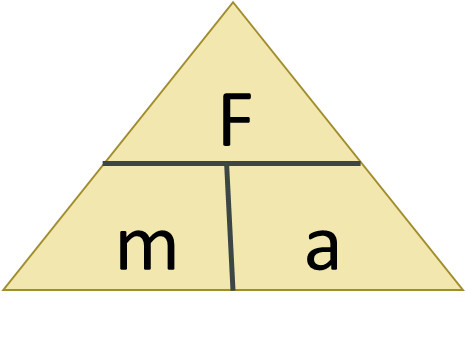
\includegraphics[scale=0.75]{Imagenes/Newton_11.jpg}
% \end{figure}
% \begin{align*}
% F = m \, a
% \end{align*}
% \end{minipage}

% Pero recordemos la expresión del tema de Movimiento Rectilíneo Uniforme, que nos relaciona la aceleración con las velocidades final e inicial junto con el tiempo.
% \begin{align*}
% a = \dfrac{v_{f} - v_{i}}{t}
% \end{align*}

% Ajustando las unidades. El valor de la velocidad se indica en \unit{\kilo\meter\per\hour}, el tiempo en el que hay un cambio de velocidad, es decir, la aceleración, se da en segundos, por lo que hay que ajustar las unidades y manejar las mismas.

% Conversión de unidades.
% \begin{align*}
% v_{i} &= \SI[per-mode=fraction]{4.5}{\kilo\meter\per\hour} \left( \dfrac{\SI{1d3}{\meter}}{\SI{1}{\kilo\meter}} \right) \left( \dfrac{\SI{1}{\hour}}{\SI{3600}{\second}} \right) = \SI[per-mode=fraction]{1.25}{\meter\per\second} \\[0.5em]
% v_{f} &= \SI[per-mode=fraction]{40}{\kilo\meter\per\hour} \left( \dfrac{\SI{1d3}{\meter}}{\SI{1}{\kilo\meter}} \right) \left( \dfrac{\SI{1}{\hour}}{\SI{3600}{\second}} \right) = \SI[per-mode=fraction]{11.11}{\meter\per\second} \\[0.5em]
% \end{align*}

% \vspace*{0.5cm}
% \textocolor{red}{Sustitución:}

% \begin{align*}
% a &= \dfrac{\SI[per-mode=fraction]{11.11}{\meter\per\second} - \SI[per-mode=fraction]{1.25}{\meter\per\second}}{\SI{8}{\second}} = \\[0.5em]
% a &= \SI[per-mode=fraction]{1.23}{\meter\per\square\second} \\[0.5em]
% F &= \left( \SI{1500}{\kilo\gram} \right) \left( \SI[per-mode=fraction]{1.23}{\meter\per\square\second} \right) \\[0.5em]
% F &= \SI[per-mode=fraction]{1845}{\kilo\gram\meter\per\square\second} = \SI{1845}{\newton}
% \end{align*}

\subsection{Tercera ley.}

% \begin{wrapfigure}{R}{0.2\linewidth}
% \centering
% \begin{figure}[H]
%     \centering
%     
\includegraphics[scale=2]{Imagenes/Pateando_Balon_02.png}
% \end{figure}
% \end{wrapfigure}
La tercera Ley de Newton indica que cuando \textocolor{denim}{un cuerpo ejerce una fuerza sobre otro}, \textocolor{red}{el segundo ejerce siempre sobre el primero una fuerza de igual magnitud pero de sentido opuesto}. A la tercera ley de Newton, se le conoce como \textocolor{auburn}{ley de acción y reacción}.

A cada fuerza de acción, le corresponde una fuerza de reacción.

\subsection*{Resumen.}

Las tres leyes de Newton son:
\begin{enumerate}
\item Ley de la inercia.
\item Ley de la relación entre la fuerza y la aceleración.
\item Ley de la acción y reacción.
\end{enumerate}

\section{Leyes de Kepler}
    
El astrónomo alemán Johannes Kepler es conocido por sus tres leyes que describen el movimiento de los planetas en sus órbitas alrededor del Sol.

\begin{figure}[H]
    \centering
    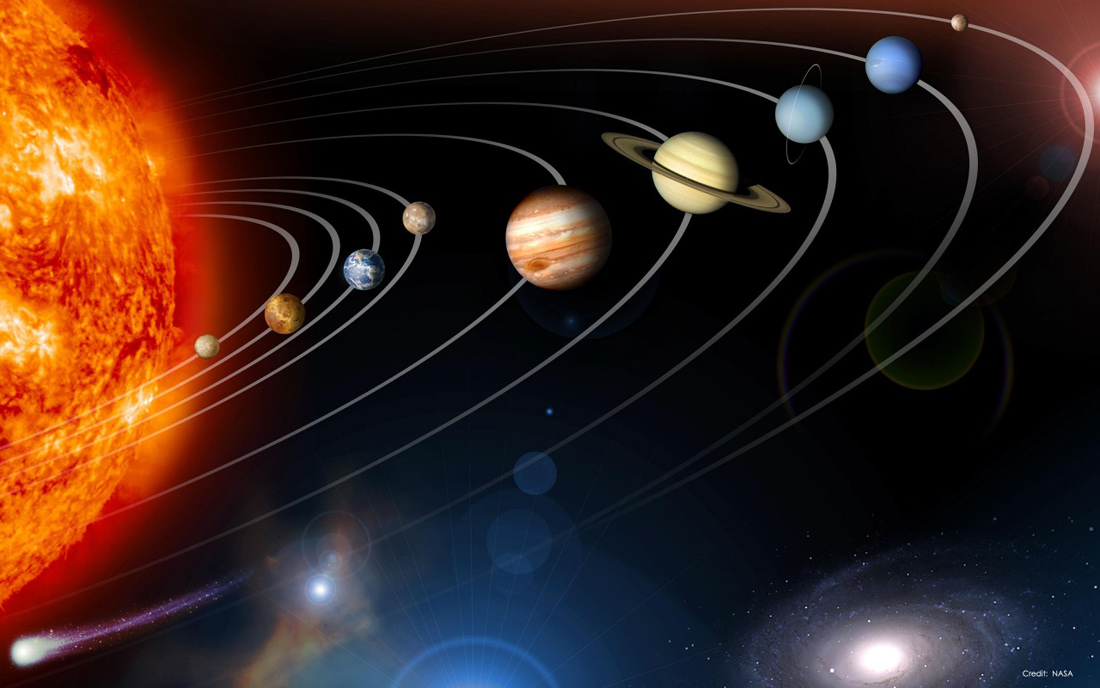
\includegraphics[scale=0.25]{Imagenes/Kepler_01.jpg}
    \caption{El Sol y los planetas del Sistema Solar.}
\end{figure}

Kepler descubrió que las \textocolor{cobalt}{trayectorias que los planetas describen alrededor del Sol eran elípticas},  basándose en lo descrito por Apolonio de Pérgamo, quien desarrolló estudios sobre la elipse.

\subsection{Primera ley.}

Todos los planetas se desplazan alrededor del Sol siguiendo \textocolor{byzantine}{órbitas elípticas}, situando al Sol en uno de sus focos.
\begin{figure}[H]
    \centering
    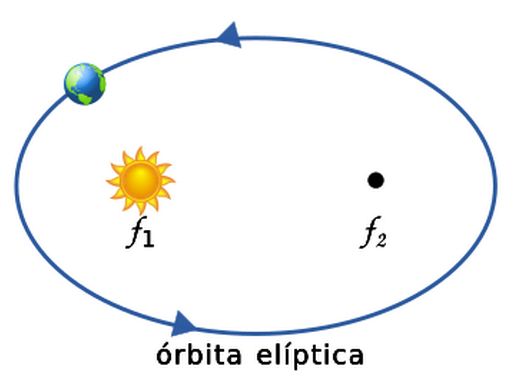
\includegraphics[scale=0.4]{Imagenes/Kepler_Leyes_01.png}
\end{figure}

En particular, hay dos puntos de interés en la órbita elíptica de la Tierra alrededor del Sol.
\begin{figure}[H]
    \centering
    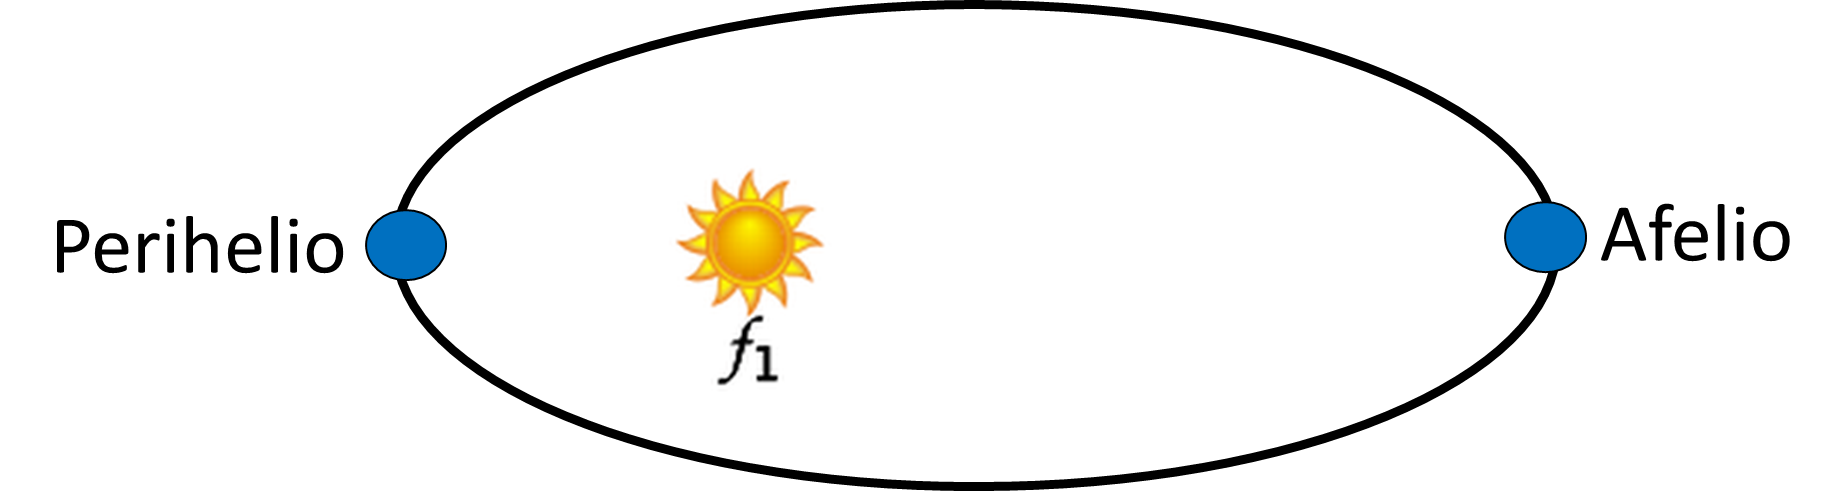
\includegraphics[scale=0.75]{Imagenes/Kepler_Leyes_01_b.png}
\end{figure}

\subsection{Segunda ley.}

La línea imaginaria que une cualquiera de los planetas con el Sol \textocolor{bulgarianrose}{barre áreas iguales en tiempos iguales}, es decir, cuando el planeta está en el \textocolor{cadmiumgreen}{afelio}, su velocidad es menor que cuando está en el \textocolor{cadmiumred}{perihelio}.
\begin{figure}[H]
    \centering
    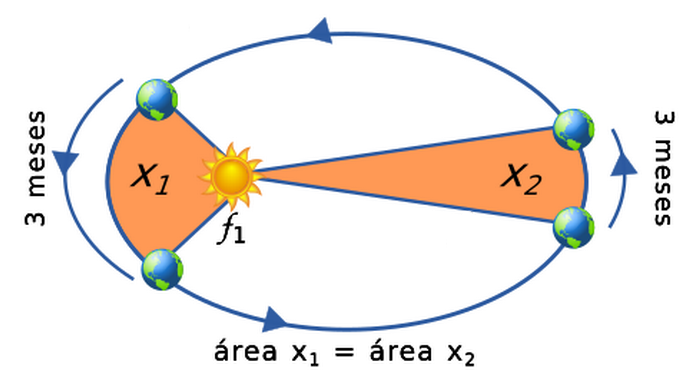
\includegraphics[scale=0.45]{Imagenes/Kepler_Leyes_02.png}
\end{figure}

Kepler demostró que los planetas tienen una mayor velocidad cuando se encuentran más cercanos al Sol que cuando están más lejanos.

\subsection{Tercera ley.}

El \textocolor{red}{cuadrado del período} ($T$) de cualquier planeta tiene una variación directamente proporcional con el \textocolor{cardinal}{cubo del radio de su órbita} ($r$), es decir, con el cubo de la distancia promedio que existe desde un planeta hasta el Sol.

Matemáticamente, se expresa con la fórmula:
\begin{align*}
T^{2} = k \, r^{3}
\end{align*}
donde $k$ es una constante de proporcionalidad, que tiene el mismo valor para todos los planetas.

\section{Los planetas del Sistema Solar.}

A continuación, se presenta una lista de los planetas del sistema solar, incluyendo información sobre su distancia al Sol, periodos de rotación sobre su eje, periodo de traslación alrededor del Sol, valor de gravedad (comparado con la gravedad terrestre), y algunas características distintivas:

\begin{enumerate}
\item \textbf{Mercurio:}

Distancia al Sol: 57.9 millones de \unit{\kilo\meter} \\
Periodo de Rotación: 58.6 días \\
Periodo de Traslación: 88 días \\
Gravedad: $g = \SI{3.72}{\meter\per\square\second}$ \\
Características: Superficie con cráteres, sin atmósfera significativa, temperaturas extremas.

\item \textbf{Venus:}

Distancia al Sol: 108.2 millones de \unit{\kilo\meter} \\
Periodo de Rotación: 243 días \\
Periodo de Traslación: 225 días \\ 
Gravedad: $g = \SI{8.92}{\meter\per\square\second}$ \\
Características: Atmósfera densa, efecto invernadero, terreno montañoso y volcánico.

\item \textbf{Tierra:}

Distancia al Sol: 149.6 millones de \unit{\kilo\meter} \\
Periodo de Rotación: 24 horas \\
Periodo de Traslación: 365.25 días \\
Gravedad: $g = \SI{9.81}{\meter\per\square\second}$ \\
Características: Único planeta con vida conocida, diversidad geográfica, atmósfera rica en oxígeno.

\item \textbf{Marte:} 

Distancia al Sol: 227.9 millones de \unit{\kilo\meter} \\
Periodo de Rotación: 24.6 horas \\
Periodo de Traslación: 687 días \\
Gravedad: $g = \SI{3.72}{\meter\per\square\second}$ \\
Características: Se le conoce como el \enquote{Planeta Rojo}, presenta montañas, cañones, posible presencia pasada de agua.

\item \textbf{Júpiter:}

Distancia al Sol: 778.5 millones de \unit{\kilo\meter} \\
Periodo de Rotación: 9.9 horas \\ 
Periodo de Traslación: 11.9 años \\
Gravedad: $g = \SI{23.15}{\meter\per\square\second}$ \\
Características: Es el planeta más grande del Sistema Solar, cuenta con un sistema de anillos, la Gran Mancha Roja es una tormenta con vientos de más de \SI{400}{\kilo\meter\per\hour}, cuenta con más de 70 lunas (satélites naturales).

\item \textbf{Saturno:}

Distancia al Sol: 1,427 millones de \unit{\kilo\meter} \\
Periodo de Rotación: 10.7 horas \\
Periodo de Traslación: 29.5 años \\
Gravedad: $g = \SI{9.02}{\meter\per\square\second}$ \\
Características: Forma un sistema de anillos espectaculares, en su atmósfera se detectan patrones de nubes, cuenta con más de 80 lunas.

\item \textbf{Urano:}

Distancia al Sol: 2,870 millones de \unit{\kilo\meter} \\
Periodo de Rotación: 17.2 horas \\
Periodo de Traslación: 84 años \\
Gravedad: $g = \SI{8.73}{\meter\per\square\second}$ \\
Características: El eje del planeta tiene una inclinación extrema, su atmósfera está formada principalmente de hidrógeno y helio, cuenta también con un sistema de anillos y lunas.

\item \textbf{Neptuno:}

Distancia al Sol: 4,498 millones de \unit{\kilo\meter} \\
Periodo de Rotación: 16.1 horas \\
Periodo de Traslación: 165 años \\
Gravedad: $g = \SI{10.98}{\meter\per\square\second}$ \\
Características: Cuenta con una gran tormenta llamada \enquote{la Gran Mancha Oscura}, también cuenta con un sistema de anillos, su atmósfera está activa.
\end{enumerate}








\end{document}